\documentclass[11pt, a4]{exam}

% Use the lucida bright fonts
\usepackage[T1]{fontenc}
\usepackage[nofontinfo]{lucidabr}
\usepackage{caption} %suppress numbering figure from caption
\usepackage{hyperref}
\usepackage{tikz}
\usepackage{subcaption} % for subfigure environment

\usepackage{multirow}
\usepackage{amsmath}
\usepackage{amssymb}
	% packages that allow mathematical formatting
\usepackage{float}
\usepackage{graphicx}
	% package that allows you to include graphics
\usepackage{caption} %note below figure
\usepackage{setspace}
	% package that allows you to change spacing

\onehalfspacing
	% text become 1.5 spaced

\usepackage{fullpage}
	% package that specifies normal margins

	% package that allows you to include graphics
%%%%%%%%%%%%%%%%%%%%%%%%%%%%%%%%%%%%%%%%%%%%%%%%%%%%%%%
%%%  Uncomment the following line to print answers  %%%
\printanswers
%%%%%%%%%%%%%%%%%%%%%%%%%%%%%%%%%%%%%%%%%%%%%%%%%%%%%%%

\title{Final Examination\\\Large PUBPOL 205}
%\title{First Midterm Examination\\\Large ECON 101\thanks{Use exam.cls version 2.3  or later for best results. Currently using version \fileversion.}}
\author{Fall 2025 S1}
\date{\today}
\begin{document}
\maketitle

\bigskip
% Header line
\noindent
Name:\enspace\hrulefill\hspace{1em}
NetID:\enspace\hrulefill\hspace{1em}
Date:\enspace\hrulefill

\vspace{0.1in}

% Double-boxed instructions
\begin{center}
  \fbox{%
    \fbox{%
      \parbox{5.5in}{%
        \vspace{0.6ex}
        Answer the questions in the spaces provided on the question sheets.
        If you run out of room for an answer, continue on the back of the page.\\[0.6ex]

        \textbf{For full credit, please write clearly with legible handwriting.}\\[0.4ex]

        \textbf{You are on your honor to answer the exam questions on your own and with no assistance of any kind.}
        \vspace{0.4ex}
      }%
    }%
  }


\addpoints

% Print the grade table
\bigskip
\gradetable[v][questions]
\bigskip
\end{center}

\newpage
\begin{questions}

\question {\bf True or False Questions:} Determine whether each statement is true or false (T/F). If multiple sentences are given, evaluate only the sentence \emph{in italics}. \textbf{A justification is required for full credit}. You will \emph{not} receive credit without one.

Here is some general advice:
\begin{itemize}
\item Write down the information given and think about what it means before you formulate a response.
\item Feel free to brainstorm in the blank space, but make sure your final response is coherent and concise.
\item Whenever possible, include a graph. Label the axes and explain what the graph shows.
\item Whenever possible, write down relevant math and explain what it means.
\item If you run out of room, continue on the back of the page or ask for extra paper.
\end{itemize}


\bigskip

\bigskip
\begin{parts}

%\part[5] When the price of a good increases, the demand of that good decreases.\answerline[False]
%\part[5]  If the price of jet fuel rises, the supply of airline flights will increase.	\answerline[False]
%\part[5]  The value of a good can be expressed in terms of the quantity of another good. \answerline[True]
%\part[5]  If the budget constraint in Figure \ref{f1} becomes steeper by pivoting around the $x$-intercept, it indicates that John would have to give up \emph{less} of $X$ to obtain an additional unit of $Y$, as $Y$ has become cheaper. \answerline[True]
%\part[5]  When a good is considered a luxury item, its demand will always be price inelastic. \answerline[False]
%\part[5]  If the price of a good increases, its total revenue will always increase as well. (Hint: Demand elasticity)  \answerline[Uncertain]
%\part[5] If income stays constant, then one's purchasing power remains constant even when prices change. \answerline[False]
%\part[5] The goal of a price ceiling is to help consumers by legally lowering the price of a good, thereby transferring some of the producer's surplus to them. Therefore, this policy always improves consumer welfare. \answerline[False]
%\part[5] The EpiPen is a life-saving device for people with severe allergies. The US manufacturer of this product has raised its price by nearly 25\% each year for almost a decade. With every 25\% increase in price, it is probable that the change in quantity demanded will exceed 25\% in magnitude.  \answerline[False]
%\part[5]   In many countries around the world, the sale of kidneys is prohibited, \emph{effectively setting a price ceiling of \$0 for kidneys.} \answerline[True]
%\part[5] Lower-income smokers are more price sensitive than higher-income smokers. For simplicity, let's assume there is only one kind of cigarette available. When policymakers introduce an excise tax (i.e., a per-unit tax) on cigarettes to control smoking, \emph{they should expect a smaller increase in tax revenue from lower-income smokers}. (Hint: recall from class that, in general, revenue refers to how much of your product is sold at a given price.)  \answerline[True]
%\part[5] Essentially, the quantity demanded on the demand curve represents a collection of all feasible bundles for consumers. \answerline[False]

%%+
%\part[5] With the introduction of the first snow blower in 1927, the demand for snow shovels presumably became more elastic.  	

%\begin{figure}[H]
%\centering
%\includegraphics[scale=0.2]{snowblower.jpeg}
%\caption{A Snow Blower}
%\end{figure}
% \answerline[True]
%%-
%%+
%\part[5]}  Duke the Service Dog consumes only two things: social time (hours) with people and dog food (kg). Assume that Duke can assign utility to any bundles of social time and food, rank them, prefers a variety of the two goods over extremes, favors more of these goods, and has transitive preferences.} \emph{Then, Duke's preferences are rational.}

%\bigskip

%\begin{figure}[H]
%\centering
%\caption{A few years ago, a DKU staff member had a dog named Duke who used to lead mindfulness sessions for DKU students}
%\caption{Duke the Service Dog}
%\includegraphics[scale=0.04]{dukedog.png}
%\end{figure}

%\part[5]  The supply of paintings by Leonardo Da Vinci, who created masterpieces like the Mona Lisa and The Last Supper and passed away in 1519, is highly inelastic. \emph{Therefore, the price of these paintings is determined by demand.} \answerline[True]
%\begin{solution}[1in]
%The supply of Da Vinci paintings will be represented by a vertical line, since no amount of price fluctuation can change them. Price is therefore wholly determined by the position of the demand curve.
%\end{solution}
%\part[5] If the price of crude oil falls and the number of people who own gasoline-fueled cars increases: \emph{the equilibrium price of gasoline will increase and the equilibrium quantity of gasoline will increase.} (Hint: Gasoline is a fuel derived from crude oil and other petroleum liquids, primarily used in vehicle engines.)
%\begin{solution}[1in]
%Due to the fall of crude oil price, supply curve shifts out. Increase in demand for gasoline-fueled cars increase the demand for gasoline because such cars and gasoline are complements. There are positive shocks to both demand and supply. Equilibrium quantity unambiguously increases but their effect on price remains uncertain and depend on the magnitudes of the shifts. 
%\end{solution}
%\part[5] According to the demand and supply model we have learned so far, \emph{an increase in the demand for toilet paper results in an increase in the supply of toilet paper.} \answerline[False]


%\part[5] We typically observe only the equilibrium point that balances supply and demand.  \answerline[True]




%\part[5]  Assume John Duke consumes two goods, Good $X$ and Good $Y$, and his preferences and budget constraint are visualized as shown below in Figure \ref{f1}. \emph{When he is at Bundle $A$, he is willing to trade away more than one unit of $Y$ for an additional unit of $X$.} \answerline[False]


%\begin{figure}[H]
%\caption{John Duke's Consumer Choice Problem} \label{f1}
%\begin{center}
%\begin{tikzpicture}[scale=1]
%\draw [thick] (0,0) -- (6,0);
%\draw [thick] (0,0) -- (0,5);
%\node [right] at (6,0) {$X$};
%\node [above] at (0,5) {$Y$};

% Existing indifference curves
%\draw [thick] (0.3,4.5) to [out=290,in=165] (3.1,1.6);

% Dashed vertical lines
%\draw[dashed](0.9,3.2)--(0.9,0);
%\draw[dashed](2.2,1.9)--(2.2,0);

% Original budget constraint line
%\draw [thick] (0,3.3) -- (5.3,0);



% Adjusted indifference curve tangent to the new budget constraint
%\draw [thick] (0.8,2.8) to [out=310,in=180] (3.2,1.2);

% Adding the slope at the point of tangency (left of point B)
% Assuming the tangent point is at approximately (1.8, 2.0)
%\draw [dashed] (1.3,2) -- (2.8,1);

% Points and labels
%\node [above] at (2.4,1.9) {$B$};
%\draw[fill] (2.2,1.92) circle [radius=0.06];
%\node [right] at (0.8,3.5) {$A$};
%\draw[fill] (0.9,3.25) circle [radius=0.06];
%\node [below] at (1.8,1.57) {$C$};
%\draw[fill] (2,1.57) circle [radius=0.06];
%\node [right] at (4.8,0.5) {$\texttt{Budget Constraint}$};

%\node [right] at (3.1,1.6) {$\tt{IC_1}$};
%\node [right] at (3.3,1.15) {$\tt{IC_2}$}; % Label for the new indifference curve


%\end{tikzpicture}
%\end{center}
%\end{figure}












%\part[5] In Figure \ref{f1}, the slope at Bundle $C$ is the same as the slope of the budget constraint. \emph{Therefore, he is indifferent between consuming Bundle $C$ and Bundle $B$.} \answerline[False]



%\part[5]  If the budget constraint in Figure \ref{f1} becomes flatter by pivoting around the $x$-intercept, \emph{this indicates that John would have to give up \emph{less} of $Y$ to obtain an additional unit of $X$.} \answerline[True]




%\part[5] If the budget constraint in Figure \ref{f1} becomes flatter by pivoting around the $x$-intercept, \emph{this indicates that John's opportunity cost of consuming $X$ has increased.} \answerline[False]




%\part[5] The following excerpt from Adam Smith's ``The Wealth of Nations,'' is often referred to as `the paradox of values.' \emph{This paradox can be explained using the concept of marginal rate of substitution:}

% \\ ``The things which have the greatest value in use have frequently little or no value in exchange; and on the contrary, those which have the greatest value in exchange have frequently little or no value in use. Nothing is more useful than water: but it will purchase scarce any thing; scarce any thing can be had in exchange for it. A diamond, on the contrary, has scarce any value in use; but a very great quantity of other goods may frequently be had in exchange for it.'' \href{https://www.adamsmithworks.org/documents/chapter-iv-of-the-origin-and-use-of-money}{\textcolor{blue}{(Book I, Chapter IV)}} (Basically, this paradox says water is very valuable but cheap whereas diamonds are less valuable than water, but expensive.)  \answerline[True]













%\part[5] During World War II, the U.S. federal government, specifically the Office of Price Administration (OPA), implemented price ceilings on many goods such as dairy, meat, coffee, cars, tires, gasoline, clothes, etc. Businesses were unable to legally raise prices, which led to shortages of these goods. \emph{This price control policy caused a leftward shift in the supply curves of these goods.} \answerline[False]




%\part[5] Jane Duke spends her income on ice cream and coffee, with coffee priced at \$1 per cup. When ice cream is priced at \$1.50 per gallon, \emph{she will purchase 2 gallons of ice cream, and her total income is \$12.}  \answerline[True]

%\begin{figure}[H]
%\centering

%\caption{Jane Duke's Consumer Choice Problem}
%\includegraphics[scale=0.4]{studyguide_icecream.png}
%\end{figure}




%\part[5]  Let's suppose the government imposes a \$15 tax on wine, and the price of wine increases by \$12. \emph{This suggests that most of the tax burden is passed on to the consumer through higher prices.}\answerline[True]

%\begin{solution}[1in]
%The price increase of \$12 out of the \$15 tax shows that the tax incidence is mostly falling on consumers. This indicates that demand for wine is relatively inelastic, meaning consumers are willing to absorb most of the price increase and continue purchasing the product despite the tax.
%\end{solution}





%\part[5] \emph{Markets allocate goods to those who have the highest willingness to pay.} \answerline[True]


%\begin{solution}[1in]
%Because demand is captured by willingness to pay, those with the higher willingness to pay will be able to purchase the good. The system allocates where the good goes to the individuals who value it most. This regime is considered efficient in economics because goods are directed toward those who derive the most benefit.
%\end{solution}



%\part[5] According to the first decision rule from producer theory, the optimal number of hours to study for a PUBPOL 205 exam is reached when the additional benefit of studying for one more hour equals the additional cost of that hour.  \answerline[True]

\part[5] According to the income expansion path shown below, both bus rides and bottled water are normal goods. \answerline[False]

\begin{figure}[H]
\centering
\includegraphics[scale=0.5]{gls_f5.3.png}
\caption{Income Expansion Path}
\end{figure}

\begin{solution}[1in]
The income expansion path connects the consumer's optimal bundles as income rises, holding prices fixed. A good is normal if its consumption rises with income and inferior if its consumption falls with income. At lower incomes the path slopes upward, so consumption of both goods rises and both are normal. At higher incomes the path bends: as income keeps rising, the consumer buys more bottled water but \emph{fewer} bus rides (for example, by switching to taxis or a car). Over that range bus rides are an inferior good, so it is not true that both goods are normal. Bottled water is normal throughout.
\end{solution}


\bigskip

\bigskip

\bigskip

\bigskip

\bigskip

\bigskip

\bigskip

\bigskip

\bigskip

\bigskip

\bigskip

\bigskip

\bigskip

\bigskip

\bigskip

\bigskip




\newpage

\part[5] The substitution effect \emph{always} affects the two goods in opposite directions. \answerline[True]

\begin{solution}[1in]
The substitution effect is the change in consumption caused only by the change in relative prices, holding utility constant. Graphically, we slide along the \emph{original} indifference curve to the point where its slope equals the new price ratio. Because indifference curves slope downward (more of either good is better), staying on the same curve means that having more of one good requires having less of the other. The consumer substitutes toward the good that has become relatively cheaper and away from the good that has become relatively more expensive, so in a two-good model the substitution effect moves the two goods in opposite directions. (With perfect complements the substitution effect is zero for both goods; it never moves them in the same direction.)
\end{solution}

\bigskip

\bigskip

\bigskip

\bigskip

\bigskip

\bigskip

\bigskip

\bigskip

\bigskip

\bigskip

\bigskip

\bigskip

\bigskip

\bigskip

\bigskip

\bigskip

\bigskip


\part[5] {When the price of a good falls, consumption of one good increases and the other decreases if they are normal.}  \answerline[False]

\begin{solution}[1in]
Suppose the price of good $X$ falls and both goods are normal.
\begin{itemize}
\item Good $X$: the substitution effect raises $X$ because $X$ is now relatively cheaper. The lower price also raises purchasing power, and because $X$ is normal the income effect also raises $X$. Both effects work in the same direction, so consumption of $X$ rises.
\item Good $Y$: the substitution effect lowers $Y$ because $Y$ is now relatively more expensive. The income effect raises $Y$ because $Y$ is normal. The two effects work in opposite directions, so consumption of $Y$ can rise, fall, or stay the same.
\end{itemize}
So the other good does not necessarily decrease. Example: with Cobb--Douglas utility $U = X^{0.5}Y^{0.5}$, the consumer always spends half of income on $Y$, so $Y = 0.5\,I/P_Y$ does not change at all when $P_X$ falls.
\end{solution}


\bigskip

\bigskip

\bigskip

\bigskip

\bigskip

\bigskip

\bigskip

\bigskip

\bigskip

\bigskip

\bigskip

\bigskip

\bigskip

\bigskip

\bigskip

\newpage
\part[5]  According to the graph below, Goods $X$ and $Y$ are substitutes, and the cross-price elasticity of demand between them is negative. \answerline[False]

\begin{figure}[H]
\centering
\includegraphics[scale=0.25]{ch5_crosselasticity.png}
\caption{When the Price of One Good Changes}

\end{figure}

\begin{solution}[1in]
The cross-price elasticity of demand for $X$ with respect to the price of $Y$ is
\[
\varepsilon_{XY} = \frac{\%\Delta Q_X}{\%\Delta P_Y}.
\]
If $X$ and $Y$ are substitutes, a rise in $P_Y$ makes consumers switch toward $X$, so $Q_X$ rises and $\varepsilon_{XY} > 0$. If they are complements, a rise in $P_Y$ lowers $Q_X$, so $\varepsilon_{XY} < 0$. The sign of the cross-price elasticity is exactly what tells us whether two goods are substitutes or complements, so ``substitutes with a negative cross-price elasticity'' is impossible. To read the graph, check how consumption of the other good responds when one good's price changes: if it moves in the same direction as the price (price up, other good up), the goods are substitutes and $\varepsilon_{XY} > 0$; if it moves in the opposite direction, they are complements and $\varepsilon_{XY} < 0$. Either way, the statement is false.
% NOTE: ch5_crosselasticity.png was not available when this solution was written.
% Replace the "To read the graph..." sentence with the case the figure actually shows.
\end{solution}
\bigskip

\bigskip

\bigskip

\bigskip

\bigskip

\bigskip

\bigskip

\bigskip

\bigskip

\bigskip

\bigskip

\bigskip

\bigskip

\bigskip


\part[5] Studying the behavioral responses of lottery winners is a good setting to examine substitution effects.  \answerline[False]

\begin{solution}[1in]
A lottery prize is a pure income shock: it raises the winner's income but leaves relative prices unchanged, including the wage (the price of leisure) and the prices of goods. The budget constraint shifts out in parallel and its slope does not change. With no change in relative prices there is no substitution effect to observe. Lottery winners are instead a good setting to study \emph{income} effects, for example how much people reduce their hours of work when they become richer. Because who wins is determined by chance among people who bought tickets, comparing winners with non-winners isolates the effect of the extra income.
\end{solution}


\bigskip

\bigskip

\bigskip

\bigskip

\bigskip

\bigskip

\bigskip

\bigskip

\bigskip

\bigskip

\bigskip

\bigskip

\bigskip

\bigskip


\part[5] Salt has inelastic demand. \emph{This means that the income effect is huge.} \answerline[False]

\begin{solution}[1in]
Inelastic demand means quantity demanded responds little to price. The income effect of a price change is large only when the good is a large share of the budget, because only then does a price increase substantially reduce purchasing power. Salt is a tiny share of spending. If salt is 0.1\% of a household's budget and its price doubles, the household's purchasing power falls by only about 0.1\%, so the income effect is close to zero. Salt's demand is inelastic because \emph{both} effects are small: the substitution effect is small because salt has few good substitutes, and the income effect is small because salt is a tiny share of the budget.
\end{solution}





\bigskip

\bigskip

\bigskip

\bigskip

\bigskip

\bigskip

\bigskip

\bigskip

\bigskip

\bigskip

\bigskip

\bigskip

\bigskip

\bigskip

\bigskip

\bigskip

\bigskip

\bigskip

\part[5] {If the average cost ($AC$) up to the 6th unit of output is \$15 and the marginal cost ($MC$) of producing the 7th unit is \$12, then the average cost ($AC$) is rising.}  \answerline[False]


%\part[5] An increase in the price of a good will cause a movement along the supply curve for that good. \answerline[True]


\bigskip


\begin{solution}[1in]
When the marginal cost of an additional unit is below the current average cost, producing that unit pulls the average down.
\[
TC(6) = 6 \times \$15 = \$90, \qquad TC(7) = \$90 + \$12 = \$102, \qquad AC(7) = \frac{\$102}{7} \approx \$14.57 < \$15.
\]
Average cost is falling, not rising. (The same logic applies to grades: if your average score is 15 and you score 12 on the next quiz, your average falls.)
\end{solution}



\bigskip

\bigskip

\bigskip

\bigskip

\bigskip

\bigskip

\bigskip

\bigskip

\bigskip

\bigskip

\bigskip

\bigskip

\bigskip

\bigskip

\bigskip

\bigskip

\newpage
\part[5] The total cost function sometimes decreases as output increases. \answerline[False]

\begin{solution}[1in]
Total cost is $TC(Q) = FC + VC(Q)$. Producing more output requires at least as much of the inputs, and inputs have nonnegative prices, so producing more cannot cost less than producing less. (A firm could always produce the larger output and discard the extra units.) Total cost is therefore nondecreasing in output, and $MC = \Delta TC/\Delta Q \geq 0$. What can fall as output increases is marginal cost (total cost rising more slowly) or average cost, but not total cost itself.
\end{solution}


\bigskip

\bigskip

\bigskip

\bigskip

\bigskip

\bigskip

\bigskip

\bigskip

\bigskip

\bigskip

\bigskip

\bigskip

\bigskip

\bigskip

\bigskip
\part[5]  The interest rate is the relative price of spending today versus spending in the future. \answerline[True]

\begin{solution}[1in]
With two periods, saving \$1 today returns $\$(1+r)$ next period, and borrowing \$1 today costs $\$(1+r)$ next period. The intertemporal budget constraint is
\[
C_1 + \frac{C_2}{1+r} = I_1 + \frac{I_2}{1+r},
\]
and with $C_1$ on the horizontal axis its slope is $-(1+r)$. Consuming one more dollar today means giving up $1+r$ dollars of future consumption, so $1+r$ is the price of present consumption in terms of future consumption, and it is set by the interest rate. For example, at $r = 5\%$, spending \$100 today costs \$105 of spending next year. A higher interest rate makes spending today more expensive relative to spending in the future.
\end{solution}


\bigskip

\bigskip

\bigskip

\bigskip

\bigskip

\bigskip

\bigskip

\bigskip

\bigskip

\bigskip

\bigskip

\bigskip

\bigskip

\bigskip

\bigskip

\newpage
\part[5] McDonald’s is replacing cashiers with touchscreen ordering kiosks. Currently, $MRTS = \frac{MPL}{MPK} = \frac{48}{32} = 1.5$. In other words, the marginal product of another cashier is 48 customers served per hour, and the marginal product of another kiosk is 32 customers served per hour. A cashier can be hired for a wage of \$15 per hour, and a kiosk rents for \$12 per hour. \emph{McDonald’s is currently minimizing the cost of serving its customers.}
 \answerline[False]

\begin{solution}[1in]
A firm minimizes cost when the last dollar spent on each input buys the same output:
\[
\frac{MP_L}{W} = \frac{MP_K}{R} \quad\Longleftrightarrow\quad MRTS = \frac{MP_L}{MP_K} = \frac{W}{R},
\]
where $W$ is the wage and $R$ is the rental price of a kiosk. Here $MRTS = 48/32 = 1.5$ but $W/R = \$15/\$12 = 1.25$, so the condition fails. Per dollar, a cashier serves $48/15 = 3.2$ customers per hour, while a kiosk serves $32/12 \approx 2.67$. Because these are not equal, McDonald's is not minimizing cost.
\end{solution}

\bigskip

\bigskip

\bigskip

\bigskip

\bigskip

\bigskip

\bigskip

\bigskip

\bigskip

\bigskip

\bigskip

\bigskip

\bigskip

\bigskip

\bigskip

\bigskip

\bigskip

\bigskip

\bigskip

\bigskip


\part[5] Continuing with the previous problem, McDonald’s should hire more workers. \answerline[True]

\begin{solution}[1in]
From the previous part, $MP_L/W = 3.2 > MP_K/R \approx 2.67$: the last dollar spent on a cashier serves more customers than the last dollar spent on a kiosk. McDonald's can serve the same number of customers at lower cost by shifting spending from kiosks to cashiers, that is, by hiring more workers and renting fewer kiosks. For example, renting one fewer kiosk saves \$12 per hour and loses 32 customers per hour. Serving those 32 customers takes $32/48 = 2/3$ of a cashier-hour, which costs $\tfrac{2}{3}\times\$15 = \$10$. Cost falls by \$2 per hour with no loss of output. As McDonald's adds cashiers and drops kiosks, $MP_L$ falls and $MP_K$ rises (diminishing marginal products) until $MP_L/W = MP_K/R$. Graphically, $MRTS = 1.5 > W/R = 1.25$ means the isoquant is steeper than the isocost line at the current input mix, so moving along the isoquant toward more labor and less capital lowers cost. At these numbers, replacing cashiers with kiosks moves in the wrong direction.
\end{solution}

\bigskip

\bigskip

\bigskip

\bigskip

\bigskip

\bigskip

\bigskip

\bigskip

\bigskip

\bigskip

\bigskip


\bigskip

\bigskip

\bigskip


\bigskip

\bigskip

\bigskip


\part[5] The long-run average total cost ($LATC$) curve always lies at the lower bound of the short-run average total cost ($SATC$) curves.
 \answerline[True]

\begin{solution}[1in]
In the long run the firm can choose all of its inputs, including its plant size (capital $K$). For any output $Q$, long-run average cost is the lowest average cost over all possible plant sizes:
\[
LATC(Q) = \min_{K} SATC(Q; K).
\]
So $LATC(Q) \leq SATC(Q;K)$ for every plant size $K$, with equality at the output for which that plant size is the cost-minimizing one. Graphically, the $LATC$ curve is the lower envelope of the $SATC$ curves: it touches each $SATC$ curve at one point and never lies above any of them.
\begin{center}
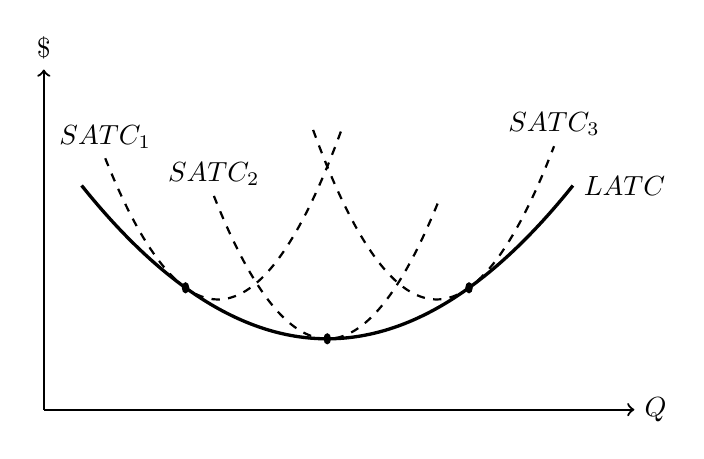
\begin{tikzpicture}[xscale=0.6, yscale=0.9]
\draw[->, thick] (0,0) -- (12.5,0) node[right] {$Q$};
\draw[->, thick] (0,0) -- (0,4.8) node[above] {$\$$};
% LATC(Q) = 1 + 0.08 (Q-6)^2; each SATC_k = LATC(q_k) + LATC'(q_k)(Q-q_k) + 0.35 (Q-q_k)^2,
% so SATC_k - LATC = 0.27 (Q-q_k)^2 >= 0, with tangency at q_k = 3, 6, 9.
\draw[very thick, domain=0.8:11.2, samples=100] plot (\x, {1 + 0.08*(\x-6)^2}) node[right] {$LATC$};
\draw[thick, dashed, domain=1.3:6.3, samples=100] plot (\x, {1.72 - 0.48*(\x-3) + 0.35*(\x-3)^2});
\draw[thick, dashed, domain=3.6:8.4, samples=100] plot (\x, {1 + 0.35*(\x-6)^2});
\draw[thick, dashed, domain=5.7:10.8, samples=100] plot (\x, {1.72 + 0.48*(\x-9) + 0.35*(\x-9)^2}) node[above] {$SATC_3$};
\node[above] at (1.3,3.55) {$SATC_1$};
\node[above] at (3.6,3.02) {$SATC_2$};
\foreach \q/\c in {3/1.72, 6/1, 9/1.72} \fill (\q,\c) circle [radius=0.08];
\end{tikzpicture}
\end{center}
Note that each tangency point is generally not the minimum of that $SATC$ curve: on the downward-sloping part of $LATC$ the tangency lies to the left of the $SATC$ minimum, and on the upward-sloping part it lies to the right.
\end{solution}


\bigskip

\bigskip

\bigskip

\bigskip

\bigskip

\bigskip

\bigskip

\bigskip

\bigskip

\bigskip

\bigskip

\bigskip


\bigskip

\bigskip

\bigskip


\end{parts}

%%%%%






\newpage




\question \textbf{Long Answer Questions.}  Concrete blocks are produced by thousands of small producers in a perfectly competitive market. Each producer faces total costs of $TC = Q^{3} - 6Q^{2} + 20Q + 300$, where $Q$ is the quantity of blocks, in hundreds. The corresponding marginal cost curve is given by $MC = 3Q^{2} - 12Q + 20$. 

\begin{parts}

\part[5]  How can the variable cost, $VC$ can be inferred from $TC$?

\begin{solution}[1in]
Fixed cost is the part of total cost that does not change with output, so it is what remains when $Q = 0$: $FC = TC(0) = 300$. Variable cost is everything that depends on $Q$:
\[
VC = TC - FC = Q^{3} - 6Q^{2} + 20Q.
\]
Check: $\dfrac{dVC}{dQ} = 3Q^{2} - 12Q + 20 = MC$, as given. The fixed cost does not affect marginal cost.
\end{solution}


\bigskip

\bigskip

\bigskip

\bigskip

\bigskip

\bigskip

\bigskip

\bigskip

\bigskip

\bigskip


\part[5]  Get $AVC$.

\begin{solution}[1in]
\[
AVC = \frac{VC}{Q} = \frac{Q^{3} - 6Q^{2} + 20Q}{Q} = Q^{2} - 6Q + 20.
\]
\end{solution}


\bigskip

\bigskip

\bigskip

\bigskip

\bigskip

\bigskip

\bigskip

\bigskip

\bigskip

\bigskip


\newpage
\part[5]  What is the quantity where $AVC$ is at a minimum.

\begin{solution}[1in]
Method 1: set the slope of $AVC$ to zero.
\[
\frac{dAVC}{dQ} = 2Q - 6 = 0 \quad\Longrightarrow\quad Q = 3.
\]
The second derivative is $2 > 0$, so this is a minimum.

Method 2: $MC$ crosses $AVC$ at the minimum of $AVC$.
\[
3Q^{2} - 12Q + 20 = Q^{2} - 6Q + 20 \;\Longrightarrow\; 2Q^{2} - 6Q = 0 \;\Longrightarrow\; 2Q(Q-3) = 0 \;\Longrightarrow\; Q = 3
\]
(ignoring $Q=0$). $AVC$ is minimized at $Q = 3$, that is, 300 blocks.
\end{solution}


\bigskip

\bigskip

\bigskip

\bigskip

\bigskip

\bigskip

\bigskip

\bigskip

\bigskip

\bigskip


\part[5]  What is the minimum price sellers must receive if they are to produce any concrete blocks at all? In other words, what is \$ of $AVC$ at that quantity?

\begin{solution}[1in]
\[
AVC(3) = 3^{2} - 6(3) + 20 = 9 - 18 + 20 = 11.
\]
Check: $MC(3) = 3(9) - 12(3) + 20 = 11 = AVC(3)$. In the short run the fixed cost of \$300 must be paid whether or not the firm produces, so a competitive firm produces only if price covers average variable cost (the shutdown rule, $P \geq \min AVC$). At any price below \$11, revenue falls short of variable cost at every output, so the firm loses more than \$300 by producing and is better off shutting down. The minimum price is therefore \$11 per unit of $Q$, i.e., \$11 per hundred blocks.
\end{solution}


\bigskip

\bigskip

\bigskip

\bigskip

\bigskip

\bigskip

\bigskip

\bigskip

\bigskip

\bigskip



\end{parts}


\newpage
\question \textbf{Long Answer Questions.} Jane Duke consumes spice and another good. She consumes 3.6 $kg$ of spice each year. Last year the price of spice doubled, and she still consumed 3.6 $kg$.






% needs: \usepackage{graphicx}

\begin{parts}

\part[5] Graph her behavior. Put spice on the $x$-axis and the other good on the $y$-axis. Draw indifference curves and budget constraints, and mark the initial and final consumption bundles.

\begin{solution}[1in]
\begin{center}
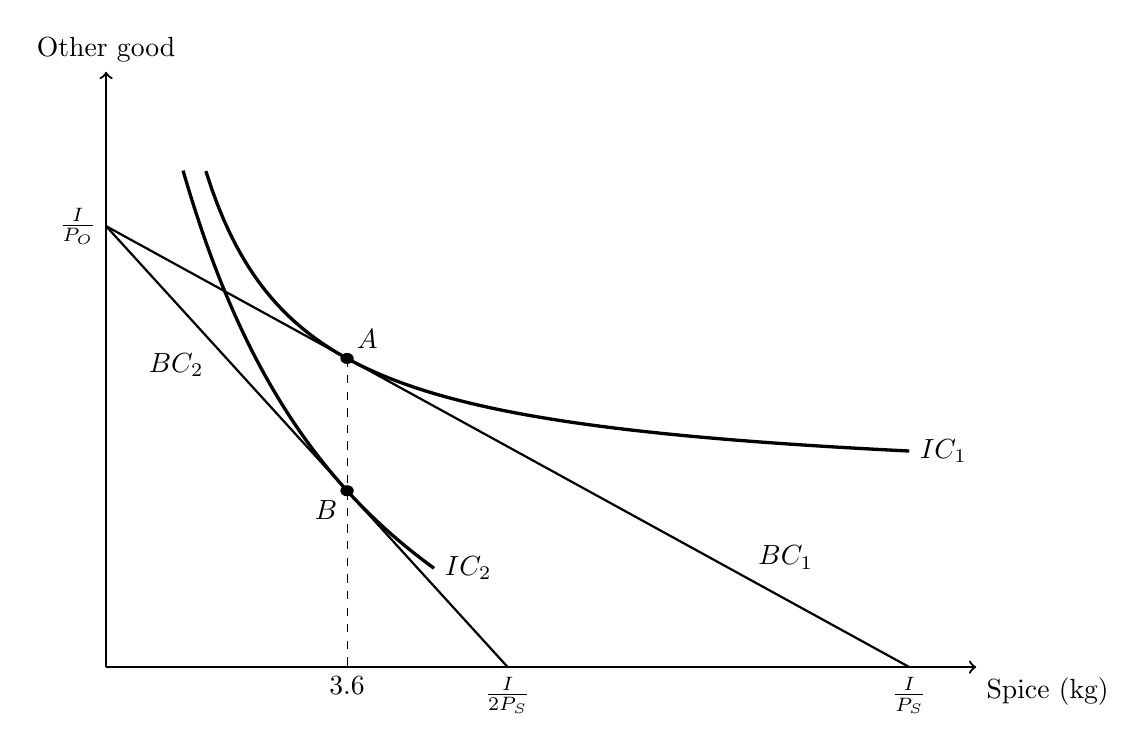
\begin{tikzpicture}[xscale=0.85, yscale=0.7]
\draw[->, thick] (0,0) -- (13,0) node[below right] {Spice (kg)};
\draw[->, thick] (0,0) -- (0,10.8) node[above] {Other good};
\draw[thick] (0,8) -- (12,0) node[below] {$\frac{I}{P_S}$};
\node[below] at (6,0) {$\frac{I}{2P_S}$};
\node[left] at (0,8) {$\frac{I}{P_O}$};
\node[above right] at (9.6,1.6) {$BC_1$};
\node[below left] at (1.6,5.87) {$BC_2$};
\draw[thick] (0,8) -- (6,0);
\draw[very thick, domain=1.49:12, samples=120] plot (\x, {3.2 + 8.64/\x}) node[right] {$IC_1$};
\draw[very thick, domain=1.15:4.9, samples=120] plot (\x, {-4.2667 + 41.8133/(\x+2)}) node[right] {$IC_2$};
\draw[dashed] (3.6,5.6) -- (3.6,0) node[below] {3.6};
\fill (3.6,5.6) circle [radius=0.1] node[above right] {$A$};
\fill (3.6,3.2) circle [radius=0.1] node[below left] {$B$};
\end{tikzpicture}
\end{center}
Let $I$ be her income, $P_S$ the original price of spice, and $P_O$ the price of the other good. When the price of spice doubles, the budget constraint rotates inward around the vertical intercept $I/P_O$ (which does not change), and the horizontal intercept falls by half, from $I/P_S$ to $I/(2P_S)$. The initial bundle $A$ is where $IC_1$ is tangent to $BC_1$ at 3.6 kg of spice. The final bundle $B$ is where the lower indifference curve $IC_2$ is tangent to $BC_2$, also at 3.6 kg. $B$ lies directly below $A$: she buys the same amount of spice, but spending on spice rises from $3.6P_S$ to $7.2P_S$, so she must consume less of the other good, and she ends up on a lower indifference curve.
\end{solution}

\bigskip

\bigskip

\bigskip

\bigskip

\bigskip

\bigskip

\bigskip

\bigskip

\bigskip

\bigskip

\bigskip

\bigskip

\bigskip

\bigskip

\bigskip

\bigskip

\bigskip

\bigskip

\bigskip

\bigskip

\bigskip

\bigskip

\bigskip

\bigskip


\newpage
\part[5] Is spice a normal or an inferior good? Explain.

\begin{solution}[1in]
Spice is an inferior good. Decompose the total change in spice consumption:
\[
\underbrace{0}_{\text{total effect}} = \underbrace{\text{substitution effect}}_{<\,0} + \underbrace{\text{income effect}}_{\text{must be}\,>\,0}.
\]
The substitution effect of a price increase is always negative: holding utility fixed, the higher relative price of spice makes her buy less of it. Because her total consumption did not change, the income effect must exactly offset the substitution effect, so it is positive. The price increase lowers her purchasing power, and this loss of purchasing power makes her buy \emph{more} spice. A good whose consumption rises when real income falls is an inferior good. (Special case: if her indifference curves had a kink at 3.6 kg, so that she wants exactly 3.6 kg regardless of prices, both effects would be zero and spice would be neither normal nor inferior. With smooth indifference curves, as drawn, spice must be inferior.)
\end{solution}

\bigskip

\bigskip

\bigskip

\bigskip

\bigskip

\bigskip

\bigskip

\bigskip

\bigskip

\bigskip

\bigskip

\bigskip

\bigskip

\bigskip

\bigskip

\bigskip

\bigskip

\bigskip

\bigskip

\bigskip

\bigskip

\bigskip

\bigskip

\bigskip



\part[5] What is her price elasticity of demand for spice?

\begin{solution}[1in]
\[
\varepsilon = \frac{\%\Delta Q}{\%\Delta P} = \frac{0\%}{100\%} = 0.
\]
(The midpoint formula gives the same answer, because $\Delta Q = 0$.) Her demand is perfectly inelastic over this price range: between $P_S$ and $2P_S$ her demand curve for spice is vertical at 3.6 kg.
\end{solution}
\bigskip

\bigskip

\bigskip

\bigskip

\bigskip

\bigskip

\bigskip

\bigskip

\bigskip

\bigskip

\bigskip

\bigskip

\bigskip

\bigskip

\bigskip

\bigskip

\bigskip

\bigskip

\bigskip

\bigskip

\bigskip

\bigskip

\bigskip

\bigskip

\part[5] Now draw the substitution and income effects in your graph from part (a).

\begin{solution}[1in]
\begin{center}
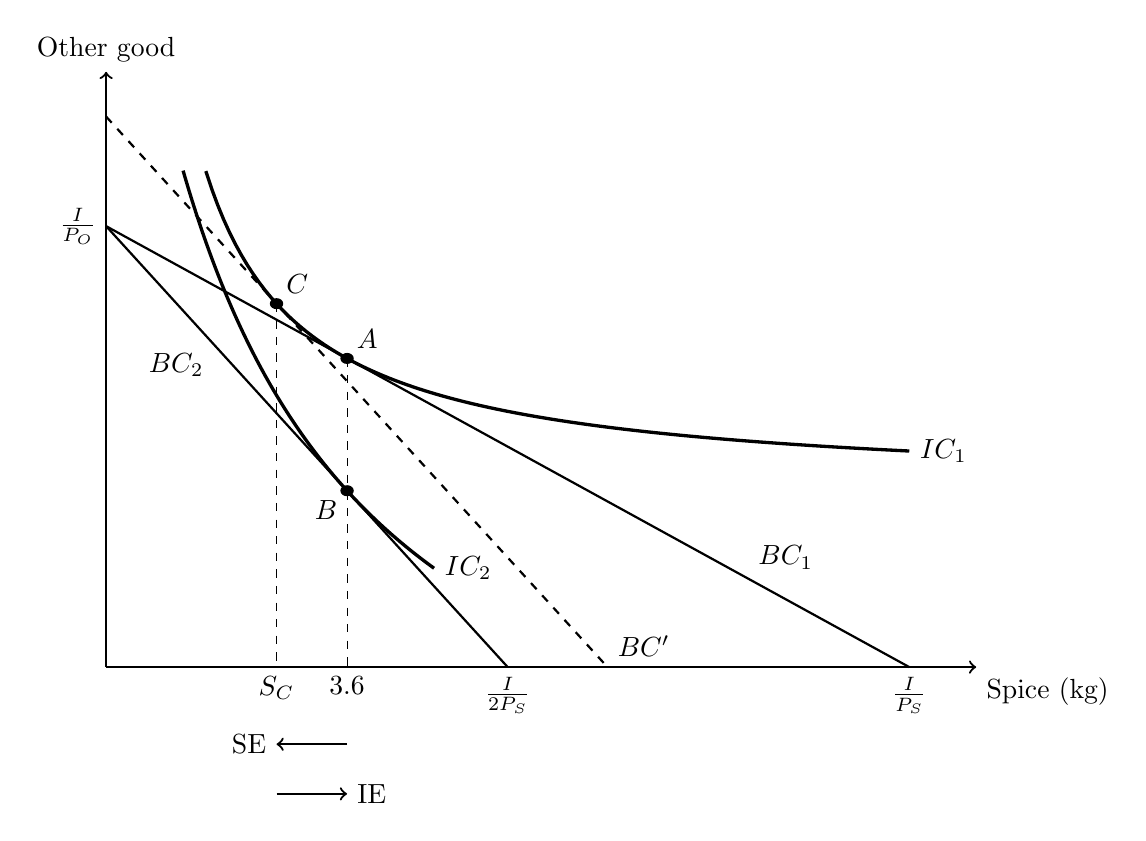
\begin{tikzpicture}[xscale=0.85, yscale=0.7]
\draw[->, thick] (0,0) -- (13,0) node[below right] {Spice (kg)};
\draw[->, thick] (0,0) -- (0,10.8) node[above] {Other good};
\draw[thick] (0,8) -- (12,0) node[below] {$\frac{I}{P_S}$};
\node[below] at (6,0) {$\frac{I}{2P_S}$};
\node[left] at (0,8) {$\frac{I}{P_O}$};
\node[above right] at (9.6,1.6) {$BC_1$};
\node[below left] at (1.6,5.87) {$BC_2$};
\draw[thick] (0,8) -- (6,0);
\draw[very thick, domain=1.49:12, samples=120] plot (\x, {3.2 + 8.64/\x}) node[right] {$IC_1$};
\draw[very thick, domain=1.15:4.9, samples=120] plot (\x, {-4.2667 + 41.8133/(\x+2)}) node[right] {$IC_2$};
\draw[dashed] (3.6,5.6) -- (3.6,0) node[below] {3.6};
\fill (3.6,5.6) circle [radius=0.1] node[above right] {$A$};
\fill (3.6,3.2) circle [radius=0.1] node[below left] {$B$};
\draw[thick, dashed] (0,9.988) -- (7.491,0) node[above right] {$BC'$};
\draw[dashed] (2.546,6.594) -- (2.546,0) node[below] {$S_C$};
\fill (2.546,6.594) circle [radius=0.1] node[above right] {$C$};
\draw[->, thick] (3.6,-1.4) -- (2.546,-1.4) node[left] {SE};
\draw[->, thick] (2.546,-2.3) -- (3.6,-2.3) node[right] {IE};
\end{tikzpicture}
\end{center}
Draw the compensated budget line $BC'$: parallel to the new budget constraint $BC_2$ (it reflects the new, higher price of spice) but shifted out just enough to be tangent to the original indifference curve $IC_1$, at bundle $C$.
\begin{itemize}
\item Substitution effect, $A \to C$: along $IC_1$, the higher relative price of spice reduces spice consumption from 3.6 kg to $S_C$.
\item Income effect, $C \to B$: the parallel shift from $BC'$ in to $BC_2$ represents the loss of purchasing power. Spice consumption \emph{rises} from $S_C$ back to 3.6 kg, which is why spice is inferior.
\item Total effect, $A \to B$: the two effects exactly offset, so spice consumption stays at 3.6 kg.
\end{itemize}
\end{solution}

\end{parts}



%%%


\end{questions}

\end{document}
